\section{Resultados}
% NOTE:
% You are expected to refer to all the floats (figures, tables, etc.)
% in the results section.
Para los resultados fue necesario recolectar dentro un TXT los datos obtenidos que eran necesarios para el análisis de complejidad. Dentro de este TXT de resultados se presentan 3 columnas. La primera columna hace referencia a la cantidad de números que se encuentran dentro del TXT que estamos leyendo. La segunda columna hace referencia a la cantidad de comparaciones realizadas durante todo el algoritmo y finalmente la tercera columna hace referencia al tiempo que se demoró el algoritmo en realizar todo el trabajo solicitado. Los resultados del experimento son los siguientes:\\

% shows how to create a table and how to refer to it

\begin{table}[H]	% uses float package to control placement
	\centering	% centers the table
	\caption{
		Resultados obtenidos y almacenados en el archivo TXT
	}	% provides a concise description of the table contents

	\begin{tabular}{r r r}
		% table header
		Tamaño & Operaciones & Tiempo transcurrido \\ 
		% inserts horizontal line
		\hline 
		% separates column entries with the ampersand &
		1000 & 3995 &  331491 \\
		1500 & 4661 &  129010 \\
		2250& 8267 &  356851 \\
		3375& 11444 & 230468 \\
		5062& 17134&  349452 \\
	    7593 & 28501 & 775948 \\
	    11389 & 36493 & 764596 \\
	    17083 & 65561 & 1147673 \\
	    25624 & 82791 & 1630712 \\
	    38436 & 135055 & 2382282 \\
	    57654 & 207684 & 4084460 \\
	    86481 & 283434 & 5366096 \\
	    129721 & 510508 & 9863766 \\
	    194581 & 604273 & 12823640 \\
	    291871 & 1064734 & 18091307 \\
	    437806 & 1505635 & 31811224 \\
	    656709 & 2208375 & 46339697 \\
	    985063 & 3732436 & 83669467 \\
	        
	\end{tabular}

	% defines a label to refer to it
\end{table}

La gráfica obtenida con estos datos es la siguiente:

\begin{figure}[H]
	% centers the figure
	\centering
	% my LaTeX installation expects Encapsulated PostScript EPS graphs
	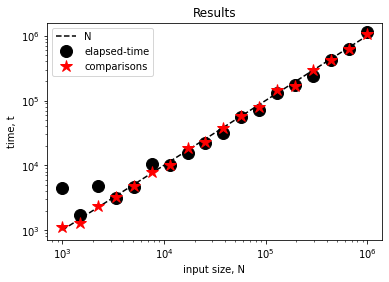
\includegraphics[keepaspectratio, width = 0.75\textwidth]{Graphic.png}
	\caption{
	  Número promedio de operaciones y tiempo de ejecución como función del tamaño del set de coordenadas.  
	}
	% defines a label to refer to it
	\label{fig:best}
\end{figure}
Como se puede observar en la gráfica, el comportamiento de los datos es claramente lineal. La línea punteada representa el comportamiento esperado para el experimento, el cuál es líneal. Los resultados obtenidos siguen el comportamiento esperado, puesto que la pendiente también corresponde a un comportamiento lineal. Los primeros datos de tiempo transcurrido difieren de lo esperado, pero estos no representan el comportamiento real del algoritmo puesto que son solo 3 datos atípicos que se deben a que las primeras ejecuciones pueden tardar más de lo esperado en lo que se normaliza su comportamiento. Otra observación importante es que algunos puntos se encuentran ligeramente por debajo o por encima de la pendiente. Esto puede deberse a que la lista de posibles candidatos es la que mayor complejidad y tiempo de ejecución añade al algoritmo puesto que utiliza la función de búsqueda por fuerza bruta a todos los candidatos que pueden ser muchos más de 3. De esta forma, si la lista de candidatos es muy grande el tiempo que se tarda en completar la tarea puede aumentar y viceversa. Esto podría ser una posible explicación para dicha variación. \\
Ahora bien, la complejidad del algortimo resulta O(n) debido a que se usa la recursividad. El algoritmo tiene 2 procesos principales, aplicar el algoritmo de fuerza bruta y encontrar los posibles puntos más cercanos (candidatos). Normalmente, el algoritmo de fuerza bruta tendría la mayor complejidad, pues el número de comparaciones sería de la forma:
\begin{align*}
    \sum_{j=i+1}^{N}{\left(
        \sum_{i=0}^{N}{1}
    \right)} =  \sum_{i=0}^{N}{N-i} = \sum_{i=0}^{N}{i} = \dfrac{N(N+1)}{2}
\end{align*}
La complejidad del método de Fuerza Bruta es claramente de $O(n^2)$ por lo que parecería que esta es la complejidad de todo el programa. Sin embargo, al dividirse el set de datos en subsets de tamaño 3 o menor, el algoritmo de fuerza bruta tendrá un N de como máximo 3. Es decir que solo hará entre 1 y 6 comparaciones, que no representan practicamente nada de complejidad tomando en cuenta que nuestro N es de más de 1000. Por ende, podemos tomar esta complejidad como O(1). Por otro lado, la subrutina que encuentra los candidatos es una búsqueda lineal del set de coordenadas. La complejidad de una búsqueda lineal es, como su nombre lo indica, lineal; O(n). Esto se demuestra ya que el número de operaciones está dado por la fórmula:
\begin{align*}
    \sum_{i=0}^{N/2-1}{1} + \sum_{i=N/2}^{N}{1} =  \sum_{i=0}^{N}{1} = N+1
\end{align*}
Esto significa que la complejidad de nuestro programa no está dictada por la complejidad del algoritmo de fuerza bruta O(1), sino por el algoritmo para hallar la lista de candidatos la cual tiene una complejidad de O(n). Por esto, nuestro programa termina con una complejidad de O(n).



